\chapter{Sparse naive Bayes}\label{ch:snb}

Naive Bayes was first introduced in the early 60s by~\cite{original_naive_bayes} for text documents classification.
Despite its naive assumptions (independence of the features),
naive Bayes remains an engaging model for large scale datasets because of its low complexity.
The time complexity to train a model is $\cO\left( n \cdot p \right)$, where $n$ and $p$ are the number of
samples and the number of features respectively.
Another appealing propriety is that naive Bayes can be trained in an online fashion,
as new data points come in a sequential order.
It can be particularly helpful if the dataset doesn't fit in memory.
Furthermore, distributed implementations could even be considered in order to speed up the learning process.

In this chapter, classical naive Bayes along with a few notations are shortly introduced.
Then, a sparse version of naive Bayes allowing in particular to perform feature selection is presented.

\section{Reminders on vanilla naive Bayes}\label{sec:naive_bayes}

In this section, we recall briefly the naive Bayes model in the specific case of binary classification,
and its training under the bernoulli, multinomial and gaussian underlying assumptions.
Most key results can naturally be extended to the multiple classes setting.

Let $n$ and $p$ be two integers, $X \in \R^{n \times p}$ a feature matrix
and $\yy \in \bset^n$ the associated target vector.
The negative and the positive classes are noted $\cC_-$ and $\cC_+$ respectively,
and will be indifferently substituted with their respective labels.

\subsection{General settings}\label{subsec:nb_general}

Note $\left( \cX,\, \cY \right)$ the pair of random variables that generated the samples and targets $X$ and $\yy$.
The goal is to explain $\yy$ given $X$, that is, finding the posterior probabilities $\Pr(\cC_\pm \mid \cX)$.
Given these probabilities, a new observation $\xx \in \R^p$ is classified according to the highest
posterior probability between the two classes
\begin{equation}\label{eq:nb_inference}
        y\left( \xx \right) = \underset{\cC \in \bclasses}{\argmax} \Pr\left( \cC \mid \xx \right)
\end{equation}
To do so, we combine the use of Bayes rule and make the (very) naive assumption that
all the features are independent given the class, that is
\begin{equation}
        \Pr\left( \cX = \xx \mid \cC_\pm \right) = \prod_{j = 1}^p \Pr(\cX_j = x_j \mid \cC_\pm)
        ,\qquad
        \Pr(\cC_\pm \mid \cX = \xx) = \frac{\Pr(\cX = \xx \mid \cC_\pm) \cdot \Pr(\cC_\pm)}{\Pr(\cX = \xx)}
\end{equation}
On the right hand side,
the denominator $\Pr(\cX = \xx)$ does not depend on the class $\cC_\pm$.
It is therefore not required to evaluate it in order to perform the inference described in~\ref{eq:nb_inference}.
Thus, we only need to estimate the probabilities $\Pr(\cC_\pm)$ and $\Pr(\xx \mid \cC_\pm)$.
The former are simply data averages, or the frequency of the positive and negative classes in the observed data.
As for the latter probabilities $\Pr\left( \xx \mid \cC_\pm \right) = \prod_{j = 1}^p \Pr(x_j \mid \cC_\pm)$,
they can be modeled by a plethora of distribution families, depending on the prior knowledge we have on the data.
The distribution is typically parametrized by some vector $\btheta \in \R^m$.
The probabilities are usually computed by maximizing the likelihood $\cL$,
or equivalently the log-likelihood $\lglh = \log\cL$, of the observed data.
\begin{equation*}
        \lglh\left( \btheta \right) = \sum_{i = 1}^n \Pr\left( \xx_i \mid y_i \,; \btheta \right)
\end{equation*}
We present now 3 meaningful cases, where the prior distributions of $\Pr(\xx \mid \cC_\pm)$ are either
gaussian, bernoulli or multinomial.
Let $\cI_\pm = \left\{ i \in \pset \mid y_i = \cC_\pm \right\}$ be the sets containing the
indexes of the positive and negative data points.
We also note for each class $\cC_\pm$ their cardinalities and empirical sums respectively, as follows:
\begin{equation*}
        n^\pm = | \cI_\pm |,
        \qquad\qquad
        \ff^\pm = \sum_{i \in \cI_\pm} \xx_i,
\end{equation*}

\subsection{Gaussian naive Bayes}\label{subsec:gnb}

In this case the observed data, conditioned on its label, is modeled by the gaussian distribution
$\cN( \bmu^\pm, \Sigma^\pm )$.
It is the most common case, to account for continuous data.
Note that the covariance $\Sigma^\pm \in \R^{p \times p}$ is diagonal because of the independence assumption that we made.
\[
        \Pr\left( \xx \mid C_\pm \right) =
        \frac{1}{\sqrt{(2\pi)^p\det(\Sigma_\pm)}}
        \exp\left( -\frac{1}{2}(\xx - \bmu_\pm)^\top\Sigma^{-1}(\xx - \bmu_\pm) \right)
\]
By denoting $\sigma_j = \Sigma_{j j}$, the log-likelihood can be written
\begin{equation*}
        \begin{split}
                \lglh_g\left( \bmu_+, \ssigma_+, \bmu_-, \ssigma_-\right ) &=
                        \sum_{j = 1}^p \Bigg[
                                \sum_{i \in \cI_+}
                                        -\frac{1}{2} \log \left( 2\pi \right)
                                        -\log \sigma_j^+
                                        -\frac{(x_j - \mu^+_j)^2}{2{\sigma^+_j}^2}\\
                                &\qquad\quad+ \sum_{i \in \cI_-}
                                        -\frac{1}{2} \log \left( 2\pi \right)
                                        -\log \sigma_j^-
                                        -\frac{(x_j - \mu^-_j)^2}{2{\sigma^-_j}^2}
                        \Bigg]
        \end{split}
\end{equation*}
The minimizer of $\lglh_g$ admits a closed-form solution:
\begin{align*}
        \bmu^\pm = \frac{\ff^\pm}{n^\pm}
        ,\qquad
        \ssigma^\pm = \sqrt{\frac{1}{n^\pm} \sum_{i \in \cI^\pm} (\xx_i - \bmu^\pm)^2}
\end{align*}

\subsection{Bernoulli naive Bayes}\label{subsec:bnb}

The Bernoulli distribution assumes that the design matrix is binary,
that is $X \in \left\{ 0, 1 \right\}^{n \times p}$.
Even though this assumption case isn't very useful in practice, its solution is simple and elegant.
Assume
In order to model the conditional probabilities, we may assume the existence of $\btheta^+, \btheta^- \in \left( 0, 1 \right)^p$
such that for any data point $\xx \in \R^p$,
\[
        \Pr\left( x_j \mid \cC_\pm \right) = (\theta^\pm_j)^{x_j} \cdot (1 - \theta^\pm_j)^{1 - x_j}
\]
It yields that $\log \Pr\left( \xx \mid \cC_\pm \right) =
\xx^\top\log\btheta^\pm + (\1 - \xx)^\top\log\left( \1 - \btheta^\pm \right)$
and finally
\begin{align}\label{eq:bernoulli_snb_ll}
        \lglh_b\left( \btheta^+, \btheta^- \right)
        &= \sum_{i \in \cI^+} \log \Pr\left( \xx_i \mid \cC_+ \right)
                + \sum_{i \in \cI^-} \log \Pr\left( \xx_i \mid \cC_- \right)\nonumber\\
        \begin{split}
                &= \ff_+^\top\log\btheta^+ + (n_+\1 - \ff_+)^\top\log\left( \1 - \btheta^+ \right)\\
                &\qquad+ \ff_-^\top\log\btheta^- + (n_-\1 - \ff_-)^\top\log\left( \1 - \btheta^- \right)
        \end{split}
\end{align}
The independence assumption makes the optimization problem decomposable across features;
it reduces to $p$ simpler maximizations, each of them admitting a closed-form solution.
Finally, we find that
\begin{equation*}
        \theta_\pm^\star = \frac{f^\pm}{n^\pm}
        ,\qquad\qquad
        \text{which is simply the average of each class.}
\end{equation*}

\subsection{Multinomial naive Bayes}\label{subsec:mnb}

Multinomial naive Bayes is more general than the Bernoulli version
as we suppose that $X \in \N^{n \times p}$ is generated by the following underlying distribution
\begin{equation*}
        \Pr\left( \xx \mid \cC_\pm \right) =
                \frac{\big( \sum_{j = 1}^p x_j \big)!}
                        {\prod_{j = 1}^p x_j!} \cdot \prod_{j = 1}^p \theta_\pm^{x_j}
\end{equation*}
It is parametrized by $\btheta^+,\, \btheta^- \in \left( 0,\, 1 \right)^p$, and they must satisfy
$\1^\top\btheta^+ = \1^\top\btheta^- = 1$ for it to be a proper distribution.
Note that this model is still valid in the more general case
where we only assume the data to be non-negative, $X \in \R_+$.
Hence, it is not as restrictive as it may appear at first sight,
as it is applicable to a large number of datasets.
The log probability is given by
\[
        \log\Pr\left(\xx \mid \cC_\pm\right) =
                \xx^\top\log\btheta_\pm + \log\frac{\big(\sum_{j = 1}^p x_j\big)!}{\prod_{j = 1}^p x_j!}
\]
and the log-likelihood reduces to
\begin{equation}\label{eq:multinomial_snb_ll}
        \lglh_m\left(\btheta^+, \btheta^-\right) = \ff_+^\top\log\btheta^+ + \ff_-^\top\log\btheta^-
\end{equation}
which is again decomposable across features.
It turns out that $\btheta_\pm^\star = \frac{\ff^\pm}{\1^\top\ff^\pm}$.

In the models presented above, the time complexity to train the naive Bayes classifier is $\cO(n \cdot p)$.
With a larger number of classes besides $\cC^-$ and $\cC^+$, say $k$ classes, this complexity is multiplied by $k$.
Besides this low asymptotic complexity,
the solutions can be computed in closed-form, which makes the effective computation cost very low.
In comparison, no closed-form solution exist for the Lasso, for logistic regression~\cite{logistic_regression},
or for SVMs~\cite{svm}.
For these models, a more costly gradient-descent based algorithm is executed to find the global optimum.

\subsection{Decision boundary}\label{subsec:nb_bound}

Given a new data point $\xx \in \R^p$, we wish to attach it the most probable label
$y \in \left\{ \cC^-,\, \cC^+ \right\}$.
No matter what model parametrized by $\btheta$ was chosen,~\ref{eq:nb_inference} reduces to
\begin{align*}
        y &= \underset{\cC \in \bclasses}{\argmax} \Pr\left( \cC \mid \xx \right)\\
        &= \sign \log \frac{\Pr(\cC^+ \mid \xx \,;\,\btheta)}{\Pr(\cC^- \mid \xx \,;\,\btheta)}\\
        &= \sign\bigg[\log \frac{\Pr(\cC^+)}{\Pr(\cC^-)}
                + \log \frac{\Pr(\xx \mid \cC^+)}{\Pr(\xx \mid \cC^-)}\bigg]
\end{align*}
In the cases of \emph{bernoulli} (\ref{subsec:bnb}) and \emph{multinomial} (\ref{subsec:mnb}) naive Bayes,
there exist $v \in \R$ and $\ww \in \R^p$ such that $y = \sign(v + \ww^\top\xx)$.
In these two special cases, the decision boundary is a hyperplane (which doesn't happen for gaussian naive Bayes).
For both of them $v$ has the same value, and by noting $\ww_b$ and $\ww_m$ the weights for the bernoulli
and the multinomial case respectively, we have
\begin{equation*}
        v = \log\frac{\Pr(\cC^+)}{\Pr(\cC^-)}
        ,\qquad
        \begin{cases*}
                \ww_b = \log(\btheta^+\odot(\1 - \btheta^-)) - \log(\btheta^-\odot(\1 - \btheta^+))\\
                \ww_m = \log\btheta^+ - \log\btheta^-
        \end{cases*}
\end{equation*}

\begin{figure}
        \centering
        \begin{subfigure}{.5\textwidth}
                \centering
                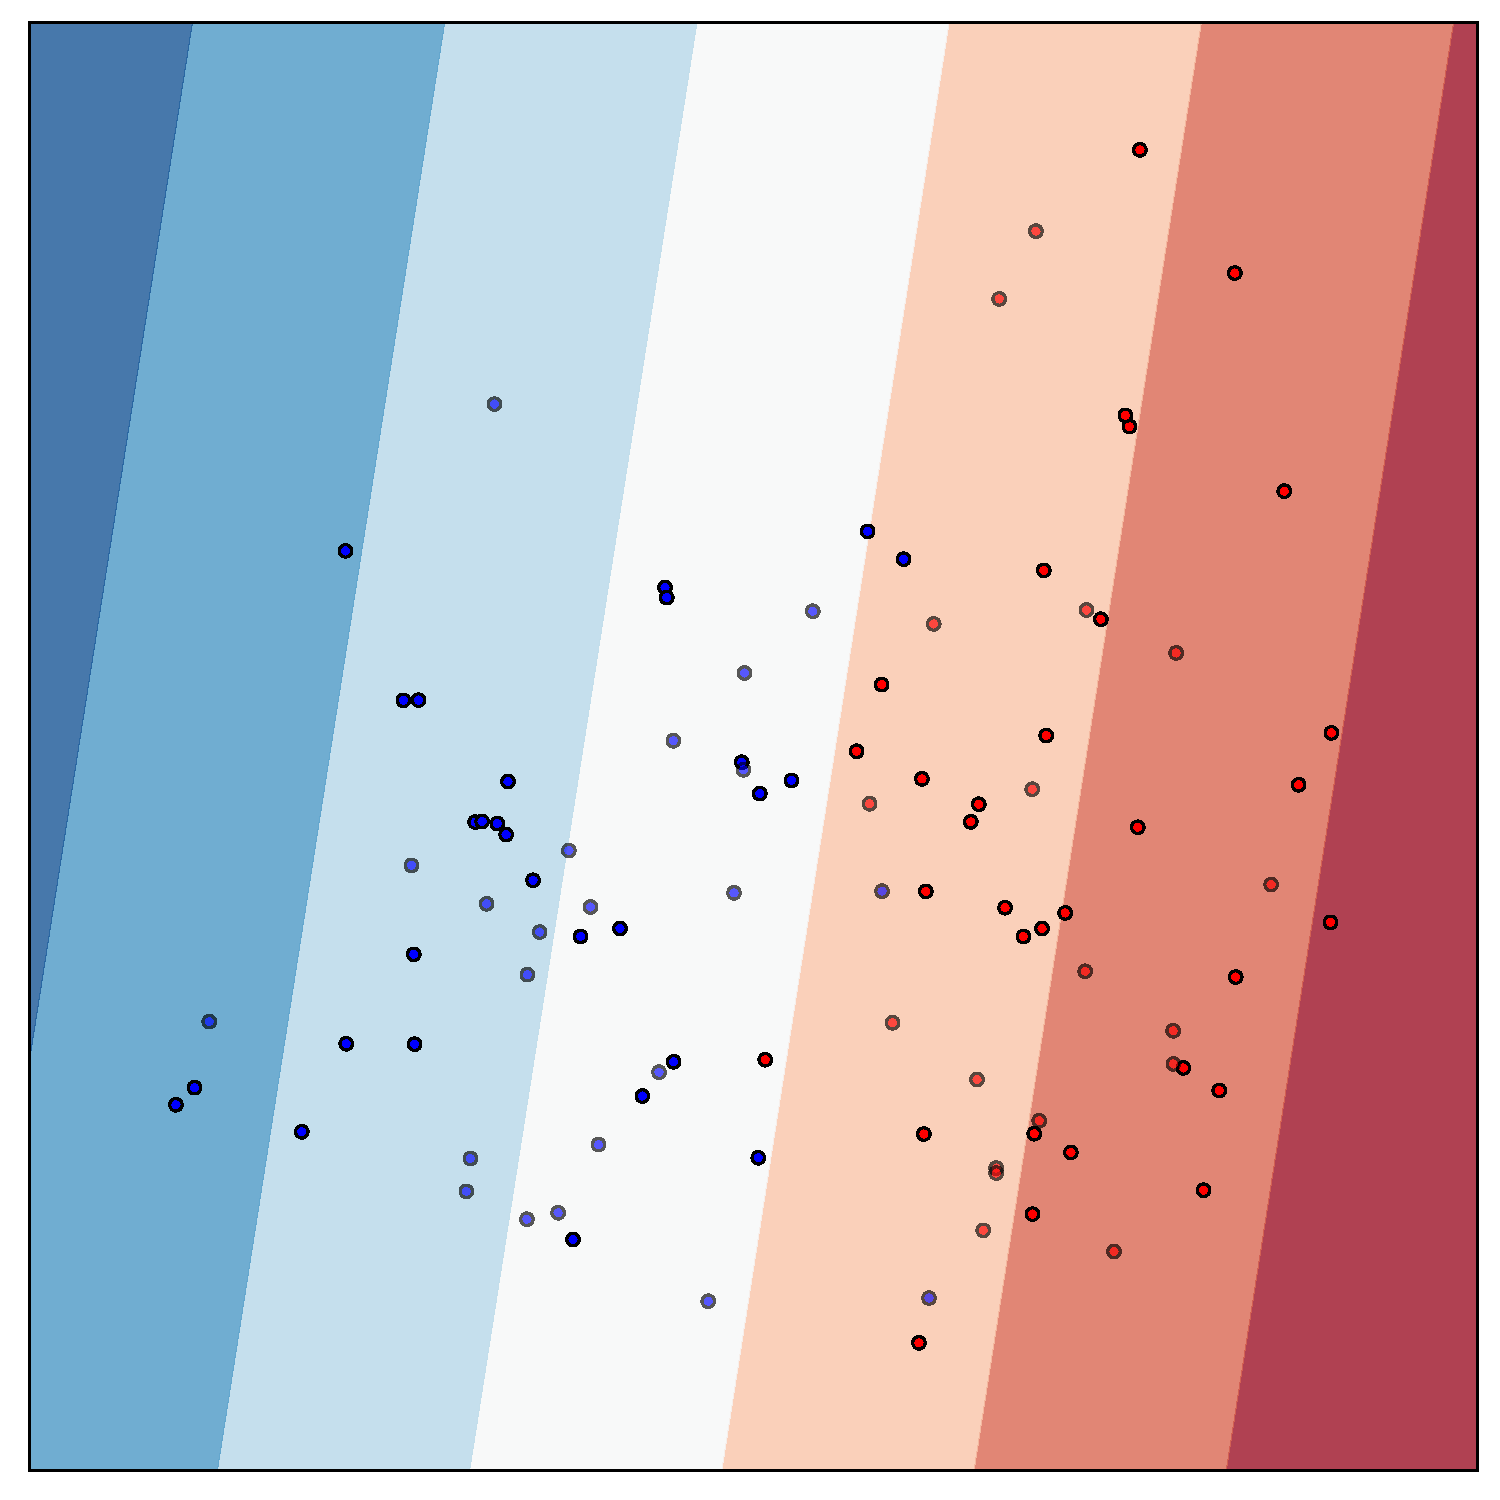
\includegraphics[width=0.75\linewidth]{figures/log_reg_classification.pdf}
                \label{fig:log_reg_classification}
        \end{subfigure}%
        \begin{subfigure}{.5\textwidth}
                \centering
                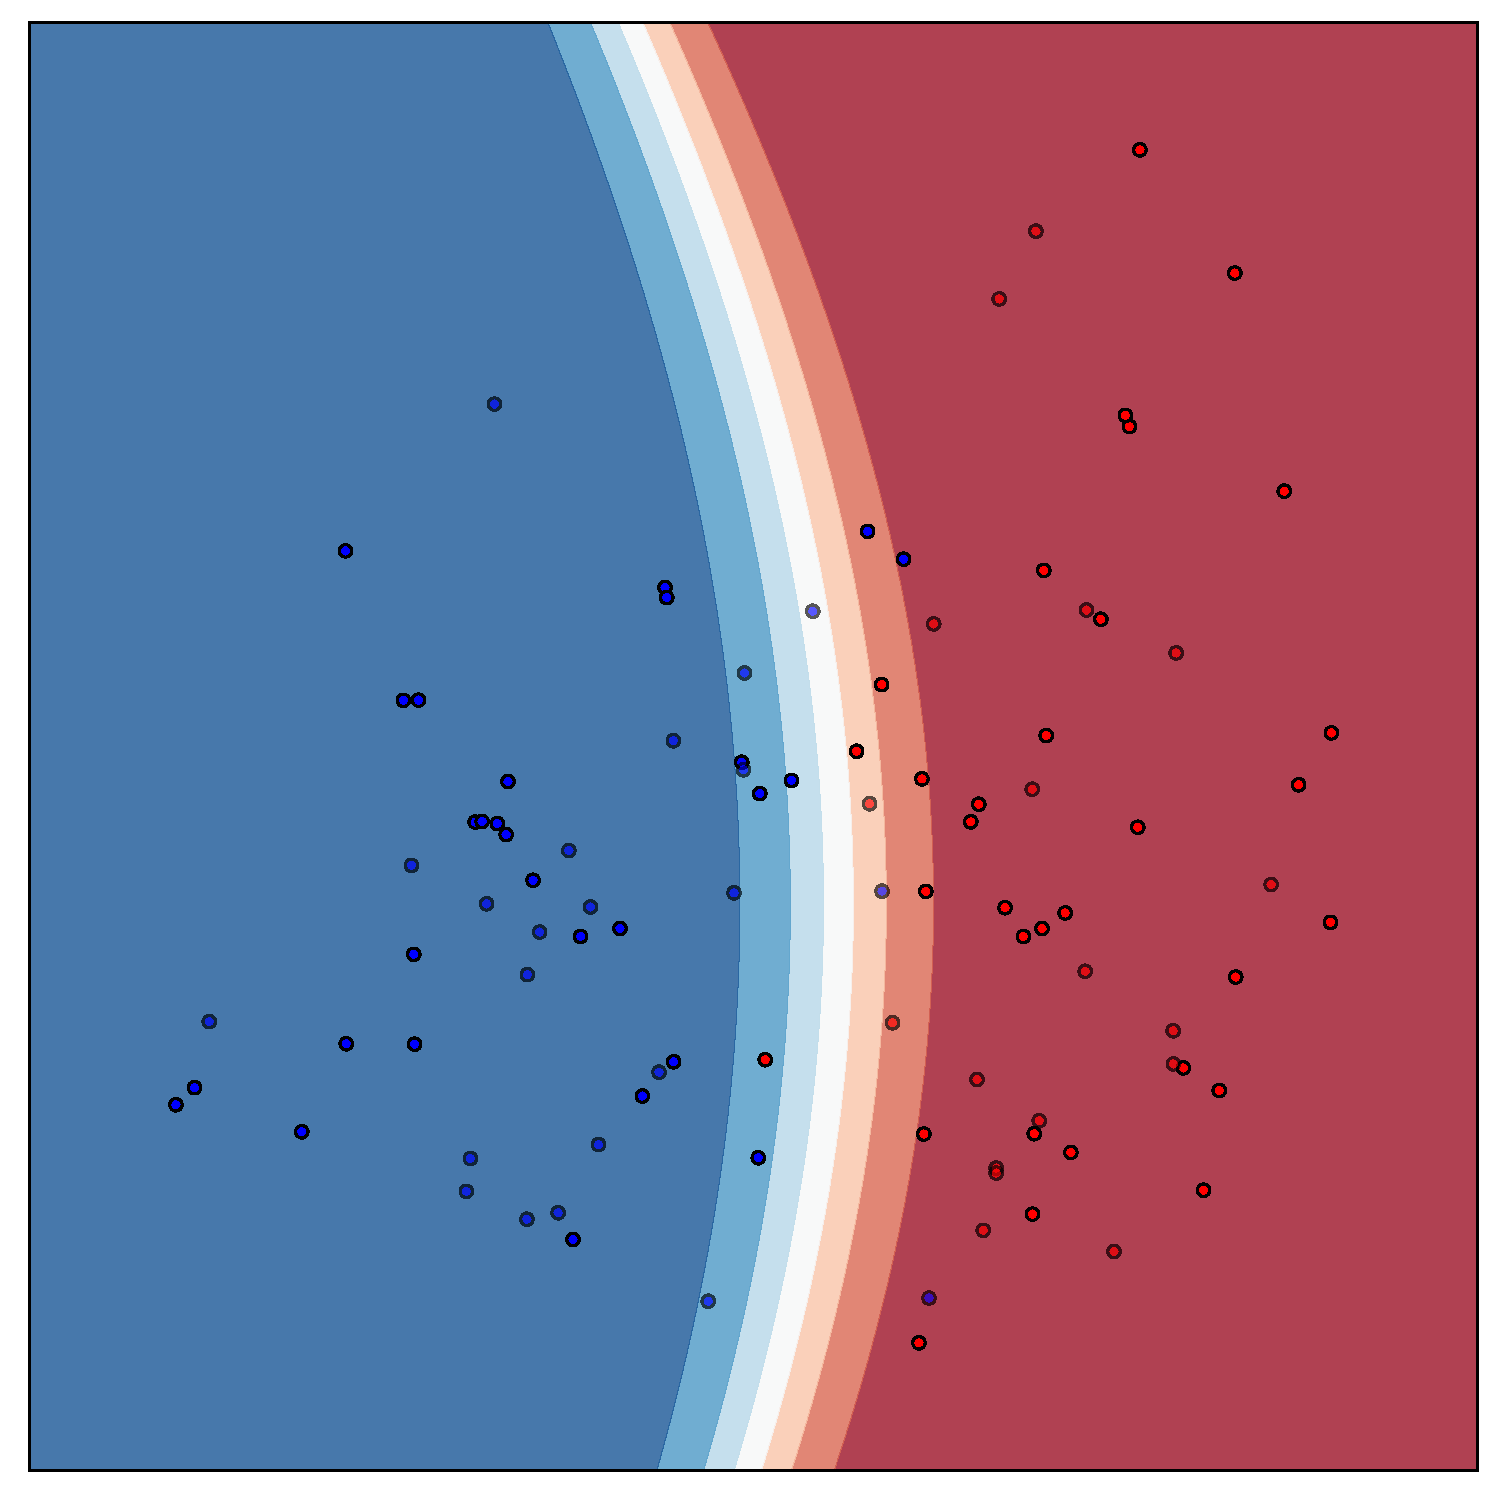
\includegraphics[width=0.75\linewidth]{figures/nb_classification.pdf}
                \label{fig:nb_classification}
        \end{subfigure}
        \caption{
                Illustration of the decision boundary for the logistic regression (left)
                and gaussian naive Bayes (right) for binary classification.
                For logistic regression, the separation is an hyperplane.
                For gaussian naive Bayes, the separation has a dependency on $x \odot x$ and can be non-linear.
                Both bernoulli and multinomial naive Bayes would have a linear separation.
        }
        \label{fig:log_reg_nb_comparison}
\end{figure}

Figure~\ref{fig:log_reg_nb_comparison} compares the decision boundary of the logistic regression to the one
of the gaussian naive Bayes.


\section{Sparse naive Bayes}\label{sec:snb}

A sparse version of naive Bayes was introduced in 2019~\cite{sparse_naive_bayes}.
They add a sparsity constraint in the Bernoulli and the multinomial optimization problems portrayed above.
It imposes the weight vector $\ww$ to have a number of non-zero entries under a certain threshold $k \in \N$.
That property is similar to the one of the Lasso presented in~\ref{subsubsec:lasso}.
But the sparsity in sparse naive Bayes (SNB) is controlled by an integer $k$,
the exact sparsity level desired on the weight vector,
while the Lasso relies on a penalty coefficient $\lambda \in \R$.
This sparsity property makes SNB employable to perform feature selection,
by keeping only the features whose weight is non-zero.
Next sections detail the problem statement, the main results of the authors,
and some applications.

\subsection{Problem statement}\label{subsec:snb_ps}


Let $0 \leq k \leq p$ be a desired level of sparsity.
We wish to train a naive Bayes classifier whose decision boundary depends on at most $k$ features.
For any $\vv \in \R^n$ we note $\norm{\vv}_0$ the number of non-zero entries
(the cardinality) of the vector.
As shown in the previous section, for both bernoulli and multinomial naive Bayes,
there exist $v \in \R$ and $\ww \in \R^p$ such that the prediction $y(\xx)$ for a new data point $\xx\in\R^p$ is
$\sign(v + \ww^\top\xx)$.
Furthermore, the $j$th entry of the decision vector $\ww$ is null if and only if $\btheta^+_j = \btheta^-_j$,
where $\btheta^+$ and $\btheta^-$ are the parameters of the loss functions $\lglh_b$ and $\lglh_m$
in~\ref{eq:bernoulli_snb_ll} and~\ref{eq:multinomial_snb_ll} respectively.
Naturally, imposing the constraint $\norm{\btheta^+ - \btheta^-}_0 \leq k$ in the optimization problems
will yield a weight vector $\ww$ with the desired sparsity.
The optimization problems for Bernoulli and multinomial SNB can be phrased as follows:
\begin{equation}\label{eq:bsnb}\tag{abc}
        \begin{aligned}
                & \underset{\btheta^+,\, \btheta^-}{\text{maximize}}
                & & \lglh_\text{b}\left( \btheta^+,\, \btheta^- \right)\\
                & \text{subject to}
                & & \norm{\btheta^+ - \btheta^-}_0 \leq k.
        \end{aligned}
        \qquad\qquad
        \begin{aligned}
                & \underset{\btheta^+,\, \btheta^-}{\text{maximize}}
                & & \lglh_\text{m}\left( \btheta^+,\, \btheta^- \right)\\
                & \text{subject to}
                & & \norm{\btheta^+ - \btheta^-}_0 \leq k\\
                & \text{ and }
                & & \1^\top\btheta^+ = \1^\top\btheta^- = 1.
        \end{aligned}
\end{equation}

\subsection{Main results and resolution}\label{subsec:snb_th}

Surprisingly, despite the combinatorial constraints,
this optimization problem can be (approximately) solved very efficiently,
with an additional minor cost compared to vanilla naive Bayes.
For the Bernoulli case especially, an optimal solution can be computed in closed-form as shown in Theorem~\ref{th:bsnb}.
\begin{theorem}\label{th:bsnb}
        Supposing that $X \in \left\{ 0, 1 \right\}^{n \times p}$ is modeled by the Bernoulli distribution.
        Then exact solution to the problem~\ref{eq:bsnb} can be computed.
        First, define $\vv$ and $\ww$ as follows
        \begin{align*}
                \mt &= (\ff^+ + \ff^-) \odot \log\left( \frac{\ff^+ + \ff^-}{n} \right)
                        + (n\1 - \ff^+ - \ff^-) \odot \log\left( \1 - \frac{\ff^+ + \ff^-}{n} \right)\\
                \begin{split}
                        \uu &= \ff^+ \odot \log \frac{\ff^+}{n^+} + (n^+\1 - \ff^+) \odot \log (\1 - \frac{\ff^+}{n^+})\\
                        &\qquad + \ff^- \odot \log \frac{\ff^-}{n^-} + (n^-\1 - \ff^-) \odot \log (\1 - \frac{\ff^-}{n^-})
                \end{split}
        \end{align*}
        Let $\cI$ be the set of $p - k$ smallest elements of $\uu - \mt$, and let
        \begin{equation*}
                {\theta^+_\star}_j = {\theta^-_\star}_j = \frac{1}{n}(f_j^+ + f_j^-)
                \;\forall j \in \cI
                ,\qquad
                {\theta^\pm_\star}_j = \frac{f^\pm_j}{n^\pm}
                \;\forall j \notin \cI
        \end{equation*}
\end{theorem}
Forming the vectors $\ff^-$ and $\ff^+$ is very quick and takes asymptotically $\cO\left( n \cdot p \right)$.
The, constructing $\mt$ and $\uu$ can be done in $\cO\left( p \right)$ steps.
Finding the $k$ largest elements of $\uu - \mt$ takes $\cO\left( p \cdot \log k \right)$ steps.
Finally, constituting $\btheta_\pm^\star$ requires $\cO\left( p \right)$ steps.
In total, the maximizer can be found in $\cO\left( n \cdot p + p \cdot \log k \right)$ steps,
which is very close to the cost $\cO\left( n \cdot p \right)$ of naive Bayes.

In the multinomial case, there is no closed-form solution, but a near-optimal one can be obtained as
stated in Theorem~\ref{th:msnb}.
\begin{theorem}\label{th:msnb}
Suppose that $X \in \R_+^{n \times p}$ is modeled by the multinomial distribution.
Define $\phi_k : \alpha \mapsto s_k(\hh(\alpha)) + C$ where $C$ is some constant,
$s_k$ the sum of the k largest values of a vector, and
\begin{equation*}
        \begin{split}
                \hh(\alpha) &= \ff_+ \odot \log \ff_+ + \ff_- \odot \log \ff_-
                                - (\ff_+ + \ff_-) \odot \log (\ff_+ + \ff_-)\\
                        &\qquad - \ff_+ \log \alpha - \ff_- \log (1 - \alpha)
        \end{split}
\end{equation*}
Let $\alpha^\star$ be the minimizer of $\phi_k$, $\cI$ the set of the $p - k$ smallest entries of
$\hh(\alpha^\star)$, and $B_\pm = \sum_{j \notin \cI} f_i^\pm$.
A primal point can be reconstructed as follows:
\[
        {\theta^+_\star}_j = {\theta^-_\star}_j = \frac{f_j^+ + f_j^-}{\1^\top(\ff^+ + \ff^-)}
        \;\forall j \in \cI
        ,\qquad
        {\theta^\pm_\star}_j = \frac{B_+ + B_-}{B_\pm}\frac{f^\pm_j}{\1^\top(\ff^+ + \ff^-)}
        \;\forall j \notin \cI
\]
Furthermore, it holds that $\psi(k - 4) \leq \phi(k) \leq \psi(k) \leq \phi(k + 4)$,
implying that the duality gap is small if $\psi(k) - \psi(k - 4)$ is small.
\end{theorem}
Experimentally, the duality gap quickly converges to $0$ as $k$ increases,
and the reconstructed primal point is near-optimal.
The time complexity is once again $\cO(n \cdot p + p \cdot \log k)$,
which is a minor additional cost compared to plain naive Bayes.

The authors experiment SNB on several text datasets,
including \textsc{amzn}, \textsc{imdb}, \textsc{twtr}, \textsc{mpqa} and \textsc{sst2}.
They compare it with more costly methods like the Lasso, $\ell_1$-penalized logistic regression and SVMs.
They obtain competitive test accuracies, while training their models several order of magnitude faster.

\section{Applications}\label{sec:nb_app}

The apparent low complexity of sparse naive Bayes compared to $\ell_1$-penalized methods such as
Lasso, logistic regression or SVMs makes is appealing for very large scale datasets.
We mention here a few applications to which we will come back later.

\subsection{Criteo dataset}\label{subsec:snb_criteo}

As part of a Kaggle competition\footnote{
        Link to the Kaggle competition: \url{https://www.kaggle.com/c/criteo-display-ad-challenge}.
}
\footnote{
        The competition's dataset can be downloaded at this address:
        \url{https://labs.criteo.com/2014/02/download-kaggle-display-advertising-challenge-dataset/}.
}
hosted by CriteoLabs in mid-2014
in Table~\ref{tab:criteo_dataset}
\begin{table}[]
        \centering
        \setlength{\tabcolsep}{2pt}
        {\small
        \begin{tabular}{|c|c|c|c|c|}\hline
        \textbf{Samples} & \textbf{Total features} & \textbf{Numerical features} & \textbf{Categorical features} & \textbf{Features after encoding}\\ \hline
        $45\,000\,000$ & $39$  & $13$ & $26$ & $10\,000\,000$ \\ \hline
        \end{tabular}
        }%
        \caption[short]{
                Criteo dataset characteristics.
                Even though the number of features is small,
                most categorical features have dozens of thousands of categories.
                It makes the training of predicting models particularly challenging as it requires several
                dozens of GB of memory.
        }
        \label{tab:criteo_dataset}
\end{table}